\paragraph{Gravitational field} $-g\hat{y}$

Examples:

\begin{align*}
Gravitational \: force \quad& \vec{F} = \underbrace{m}_{\parbox{2cm}{\scriptsize  \centering gravitational\\ mass}} \cdot \underbrace{(-g\hat{y})}_{\parbox{1.6cm}{\scriptsize  \centering at Earth's\\ surface}} \\
Electircal \: force \quad& \vec{F} = q\vec{E} \\
\end{align*}

\paragraph{Solution of movement equations} 
 \begin{align*}
x = & x_0 + (v_0 \cos \theta)t  \\
y = & y_0 + (v_0 \sin \theta)t - \frac{1}{2}gt^2\\
\end{align*}

Equation of the form of trajectory:

$$y-\left( y_0 + \frac{v_0^2 \sin^2 \theta}{2g} \right) = -\frac{g}{2v_0^2\cos^2\theta} \cdot \left[ x - \left( x_0 + \frac{v_0^2 \sin\theta \cos \theta}{g} \right) \right]$$

Maximal height:

$$h_{max} = y_m - y_0 = \frac{v_0^2 \sin^2 \theta}{2g}$$

It's possible to get it from energy too:

$$\frac{1}{2}mv_0^2 = \frac{1}{2}mv^2+mgh$$

$$\frac{1}{2}m(v_{0x}^2+v_{0y}^2) = \frac{1}{2}m(v_x^2+v_y^2)+mgh$$

$v_x=v_{0x} = const$ and $v_y=0$

$$\frac{1}{2}mv_{0y}^2= mgh$$

$$\frac{v_{0y}^2}{2g}= h$$

Range (horizontal distance when returning to same height):

$$R = \frac{2v_0^2\sin\theta\cos\theta}{g}=\frac{v_0^2\sin2\theta}{g}$$

Max range:

$$R \stackrel{\theta = \frac{\pi}{4}}{=} \frac{v_0^2}{g}$$

\subsection{Gravitational law of Newton}

Force between 2 masses:

$$\vec{F} = -\hat{r} \frac{G m_1 m_2}{r^2}$$

$G = 6.67 \cdot 10^{-11} \frac{Nm^2}{kg^2} = 6.67 \cdot 10^{-8} \frac{dyn \cdot cm^2}{g^2}$ 

\paragraph{Electromagnetic force}

\begin{align*}
Electrical \: force \quad&\vec{F} = q \vec{E} = \hat{r} q \frac{kQ}{r^2} \\
Magnetic \: force \quad&\vec{F} = q \vec{V} \times \underbrace{\vec{B}}_{\parbox{1cm}{\scriptsize  \centering magnetic\\ field}} \\
\end{align*}

$Field = \frac{force}{charge}$

\resizebox{\linewidth}{!}{ \centering
\begin{tabular}{c|c|c|c}
	Interaction&Particle&Mass& Influences on \\ \hline
	Gravitation&graviton(?)&0&Planets and stars\\\hline
	&$z^0$&99$m_p$&\\
	Weak&$w^+$&88$m_p$&decay of neuron\\
	&$w^-$&88$m_p$&\\\hline
	Electromagnetism&photon&0&Most of interactions\\\hline
	Strong&gluon&0&Protons in core\\\hline
	
\end{tabular}
}

\paragraph{Work}

Work is change of energy. Denote energy as $H$, work in one dimension $x$. $F$ is force, then

$$dH = dx F_x$$

Multiply and divide by small time:

$$dH = \frac{dx}{dt} F_x dt = \frac{dx}{dt} d p_x$$

$F_x dt = dp_x$ - is impulse

Divide by $dp_x$

$$\frac{dH}{dp_x} = \frac{dx}{dt}$$

\section{Frames of reference}

Two first laws of Newton are valid only in non-accelerating (inertial) frame of reference.
Examples of accelerating frames of references:
\begin{itemize}
	\item carousel
	\item accelerating car
\end{itemize} 

Denote inertial system as ($I$)

\paragraph{Results:}
\begin{itemize}
	\item In accelerating system body is in rest if force is on it giving him acceleration opposite to acceleration of system
	\item Inertial system is defined as system in which a body for which $\vec{F}=0$ has $\vec{a}=0$, where $\vec{a}$ is relative to the system.
\end{itemize} 

\paragraph{Imaginary forces}
Second law of Newton:
$\vec{F}=m\vec{a}_I$

$a$ - acceleration of non-inertial system 

$a_0$ - acceleration of a particle of mass $m$ in accelerating system.

$$a_I = \vec{a}+\vec{a}_0$$

$$\vec{F}_I = m \vec{a}_I = m(\vec{a}+\vec{a}_0) $$


$$\vec{F}_I - m\vec{a}_0  = m\vec{a} $$

Imaginary force: $\vec{F}_0 = -m \vec{a}_0$

Acceleration of a particle relative to accelerating system:

$$m \cdot \underbrace{\vec{a}}_{\parbox{2cm}{\scriptsize  \centering acceleration\\ in non-inertial system}} = \underbrace{\vec{F}_I}_{\parbox{2cm}{\scriptsize  \centering real force\\ exerted by car}} + \underbrace{\vec{F}_0}_{\parbox{2cm}{\scriptsize  \centering imaginary force\\ not exerted by car}}$$

\paragraph{Example} An elevator accelerating with acceleration $a_1$. $a_0=a_1$ is acceleration of the system

\begin{center}
	\includegraphics[width=0.15\linewidth]{./lect5/pic1.png}
\end{center}

Relative to elevator a person has no acceleration: $\vec{a} = 0$.

$$m\vec{a} = \vec{F}_I + \vec{F}_0$$

$$\vec{a} = 0$$

$$F_I = N-\underbrace{m}_{\parbox{2cm}{\scriptsize  \centering gravitational\\ mass}}\cdot g$$

$$F_0 = -\underbrace{m}_{\parbox{1cm}{\scriptsize  \centering inertial\\ mass}}\cdot a_1$$ %(????)

$$0=N-mg-ma_1$$

$$N=m(g+a_1)$$

We can't distinguish between acceleration of elevator and increase of free-fall acceleration, i.e. gravitational field and acceleration. Same for free-fall and lack of gravitational field.

\paragraph{Numerical example for elevator}

Elevator accelerates with $\vec{a}_1=-9.8 ms^{-2}$. Then $N=m(g+a_1)=m(9.8-9.8) = 0$, i.e. you fill weightlessness.

\paragraph{Example} Rotating system.
$\vec{\omega}$ is angular velocity perpendicular to the surface of rotation (right hand), i.e. $\odot$

\begin{center}
	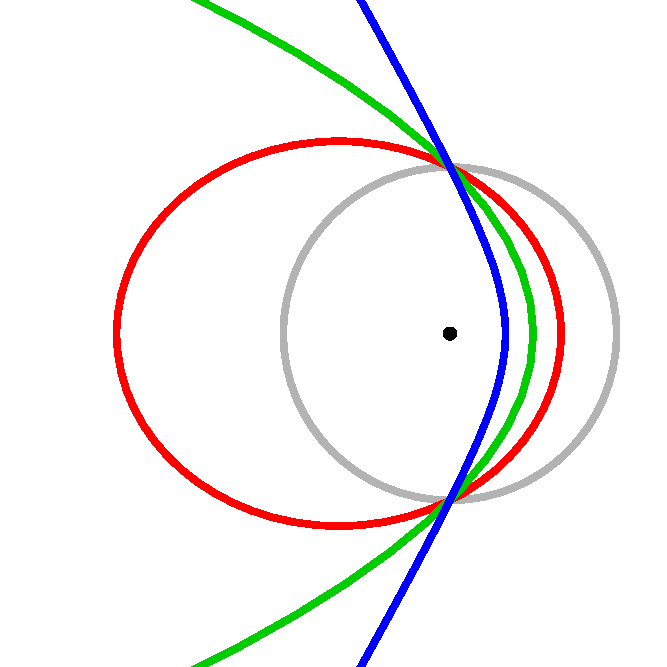
\includegraphics[width=\linewidth]{./lect5/pic2.png}
\end{center}


Mass $m$ is in rest relative to rotating system. $\vec{a}_R = 0$ and $\vec{v}_R = 0$

In inertial system it has tangent velocity: $\vec{v}_I = v_I \hat{\theta}$. $\vec{v}_I = \omega r$. $r$ is distance from center of the system. Since $\vec{v}_I \perp \vec{\omega} \perp \vec{r}$:

$$\vec{v}_I = \vec{\omega} \times \vec{r}$$

From an expression for acceleration in polar coordinates:

$$\vec{a}_I = -\hat{r}\omega^2 r = -\hat{r} \frac{v_I^2}{r}$$

$$F_I = m \vec{a}_I$$

In rotating system:

$$m\vec{a} = \vec{F}_I + \vec{F}_0$$

Since $\vec{a} = 0$

$$0m = (-\hat{r} \omega^2 r m) + \vec{F}_0$$

$$\vec{F}_0 = + \hat{r} m \omega^2 r$$

$F_I$ is centripetal force - real force inside.

$F_0$ is centrifugal force - imaginary force out.

